\documentclass{article}
\usepackage{polski}
\usepackage{babel}
\usepackage{graphicx}
\usepackage[margin=1in]{geometry}
\documentclass{article}
\usepackage[utf8]{inputenc}
\usepackage{amsmath}
\usepackage{polski}
\usepackage{babel}
\usepackage{hyperref}
\usepackage{graphicx}
\renewcommand{\figurename}{Wykres}
\title{\vspace{4cm} \textbf{Projekt ze \\ Projektowania Efektywnych Algorytmów}}
\author{Jakub Grelowski - 262754 \\
        grupa K00-58e \\
        środa - 11:15}
\date{23 listopada 2022}



\begin{document}

\maketitle

\begin{center}

\large prowadzący: dr inż. Jarosław Mierzwa 

\vspace{1cm}

\Large \textbf{\textit{Zadanie projektowe nr 1 \\ \vspace{1cm} Rozwiązanie problemu komiwojażera za pomocą przeglądu zupełnego oraz metody podziału i ograniczeń}}     
\end{center}

\vspace{1cm}

\newpage

\tableofcontents

\newpage

\section{Wstęp}
\subsection{Cel projektu}
Celem projektu było napisanie programu umożliwiającego zbadanie złożoności obliczeniowej algorytmów dokładnych rozwiązujących asymetryczny problem komiwojażera. 

\subsection{Sposób przechowywania grafów}
\begin{itemize}
    \item Macierz incydencji
\end{itemize}
\subsection{Testowane algorytmy}
\begin{itemize}
    \item Przegląd zupełny (ang. Brute force) - złożoność $O(n!)$
    \item Metoda podziału i ograniczeń (ang. Branch and bound) - złożoność $O(n^2)$
\end{itemize}

\subsection{Implementacja}
Do wykonania projektu wykorzystany został język C\# oraz środowisko programistyczne .NET Framework w wersji 4.8.


\section{Reprezentacja grafu w komputerze}
Istnieje kilka różnych sposobów reprezentacji grafu w pamięci komputera. W ramach projektu wykorzystana została macierz incydencji
\subsection{Macierz incydencji}
Macierz incydencji jest macierzą kwadratową o boku $V$, w której wartość $i$–tego wiersza i $j$–tej kolumny jest równa wadze krawędzi $A_{ij}$. Jeśli między dwoma wierzchołkami nie występuje krawędź, wartość na indeksach reprezentujących ją przyjmuje umownie $\infty$, która w programie jest reprezentowana przez 0 bądź -1.




\section{Problem komiwojażera}
Problem komiwojażera to problem obliczeniowy polegający na znalezieniu w grafie cyklu Hamiltona o najmniejszej wadze. Cykl Hamiltona to taki cykl, w którym każdy wierzchołek pojawia się dokładnie raz. 

\subsection{Asymetryczny problem komiwojażera}
Kiedy przeszukiwany graf jest skierowany - czyli waga ścieżki z punktu $A$ do punktu $B$ jest taka sama jak waga ścieżki z punktu $B$ do punktu $A$
 - mówimy wtedy o symetrycznym problemie komiwojażera. Tematem projektu jest jednak asymetryczny problem komiwojażera, czyli sytuacja przeciwna - waga ścieżki z punktu $A$ do punktu $B$ nie jest równa wadze ścieżki z punktu B do punktu A.



\newpage

\section{Algorytmy}
\subsection{Przegląd zupełny}
Przegląd zupełny polega na sprawdzeniu każdego możliwego rozwiązania. W przypadku problemu komiwojażera rozwiązań jest tyle, ile możliwych jest różnych kombinacji wierzchołków. Tak więc jeśli mamy $N$ wierzchołków, algorytm będzie musiał sprawdzić $N!$ różnych kombinacji tych wierzchołków, po czym wybrać ścieżkę z najmniejszą wagą.

\subsubsection{Implementacja}
W implementacji przeglądu zupełnego największą trudnością było generowanie nowych kombinacji. W tym celu wykorzystany został porządek leksykograficzny. W trakcie działania algorytm generuje leksykograficznie większą permutację od poprzedniej. Żeby tak zrobić, najpierw przeszukując od przedostatniego wierzchołka szukamy pierwszego wystąpienia takiego, że $A[i] < A[i+1]$. Następnie w podzbiorze po prawej szukamy pierwszej wartości mniejszej od $A[i]$. Następnie zamieniamy tą wartość z $A[i]$ i odwracamy kolejność wartości pomiędzy nimi. 


\subsubsection{Krok po kroku}
\begin{enumerate}
    \item Wygeneruj początkową permutację (wszystkie wierzchołki poza startowym).
    \item Oblicz wartości ścieżki obecnej permutacji (uwzględniając wierzchołek startowy na początku i końcu ścieżki).
    \item Jeśli obecna waga jest mniejsza od poprzedniej, zapamiętaj ją oraz ścieżkę.
    \item Wygeneruj kolejną permutację.
    \item Jeśli nie istnieje następna permutacja, zwróć ostatnio zapisaną ścieżkę oraz wagę. Jeśli istnieje, powtórz kroki 2-4.
\end{enumerate}


\subsection{Metoda podziału i ograniczenia}
Metoda podziału i ograniczenia polega na analizie drzewa przestrzeni stanów. W przypadku problemu komiwojażera stany będą reprezentować wszystkie możliwe ścieżki w grafie. By algorytm był mniej kosztowny, każdy wierzchołek drzewa posiada ograniczenie, na podstawie którego można oszacować, czy jest on obiecujący.  

\subsubsection{Implementacja}
By sprawdzić, czy przejście do konkretnego wierzchołka jest obiecujące, należy dokonać \textit{redukcji macierzy kosztów}. Oznaczamy wszystkie wartości w wierszu o indeksie wierzchołka z którego wychodzimy oraz w kolumnie o indeksie wierzchołka do którego wchodzimy jako $\infty$ (czyli -1). Następnie należy w każdym wierszu macierzy znaleźć najmniejszą wartość różną od nieskończoności i potem odjąć tą wartość od każdego elementu wierszu. Tą samą czynność powtarzamy następnie dla każdej kolumny.  Następnie dodajemy wcześniej znalezione najmniejsze wartości kolumn oraz wierszy. Ta operacja daje nam zredukowaną macierz oraz koszt jej redukcji. Programie stany są przechowywane w kolekcji przechowującej struktury składające się z zredukowanej macierzy, ścieżki oraz wagi tej ścieżki (koszty redukcji, przejścia oraz poprzednich redukcji).

\newpage
\subsubsection{Krok po kroku}
\begin{enumerate}
\item Wstępna redukcja macierzy.
\item Wyznaczenie potencjalnych kolejnych wierzchołków.
\item Dla każdego potencjalnego wierzchołka:
\begin{enumerate}
\item Redukcja macierzy kosztów.
\item Obliczenie kosztu przejścia do następnego wierzchołka.
\item Zapisanie stanu.
    \end{enumerate}

\item Znalezienie dolnej granicy.
\item Jeśli ścieżka z najmniejszą wagą ma długość końcowej ścieżki, zwróć ją. Jeżeli nie, powtórz kroki 2-4 korzystając z znalezionej granicy.
\end{enumerate}


\subsubsection{Przykład praktyczny}

\begin{center}

Przykładowa macierz:

\begin{matrix}
-1 & 2 & 5 & 3 \\
3 & -1 & 6 & 2 \\
1 & 4 & -1 & 4 \\
2 & 1 & 3 & -1
\end{matrix}

    
\end{center}




\vspace{.5cm}

Rozpoczynamy początkową redukcję: 
\newline
$
\begin{matrix}
-1 & 2 & 5 & 3 & | (-2)\\
3 & -1 & 6 & 2 & | (-2) \\
1 & 4 & -1 & 4 & | (-1) \\
2 & 1 & 3 & -1 & | (-1) 
\end{matrix}
$
\hspace{2cm}
$
\begin{matrix}
-1 & 0 & 3 & 1 \\
1 & -1 & 4 & 0 \\
0 & 3 & -1 & 3 \\
1 & 0 & 2 & -1 \\
\textunderscore & \textunderscore & \textunderscore & \textunderscore \\
0 & 0 & -2 & 0
\end{matrix}
$
\hspace{2cm}
\begin{matrix}
-1 & 0 & 1 & 1 \\
1 & -1 & 2 & 0 \\
0 & 3 & -1 & 3 \\
1 & 0 & 0 & -1
\end{matrix}




\vspace{.75cm}
\begin{center}
Początkowy koszt: $2 + 2 + 1 + 1 + 2 = 8$    
\\ \vspace{.1cm}
Dostępne do odwiedzenia wierzchołki:
\end{center}

\begin{figure}[h]
    \centering
    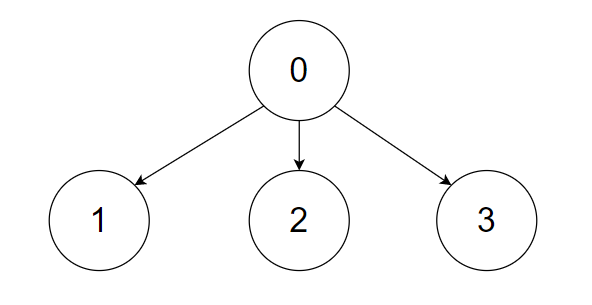
\includegraphics[scale=0.45]{img/graf1.png}
\end{figure}

\newline

\begin{center}
Po zredukowaniu (na czerwono zaznaczono pozycje oznaczone jako $\infty$ w trakcie redukcji):    
\end{center}


\begin{figure}[h]
    \centering
    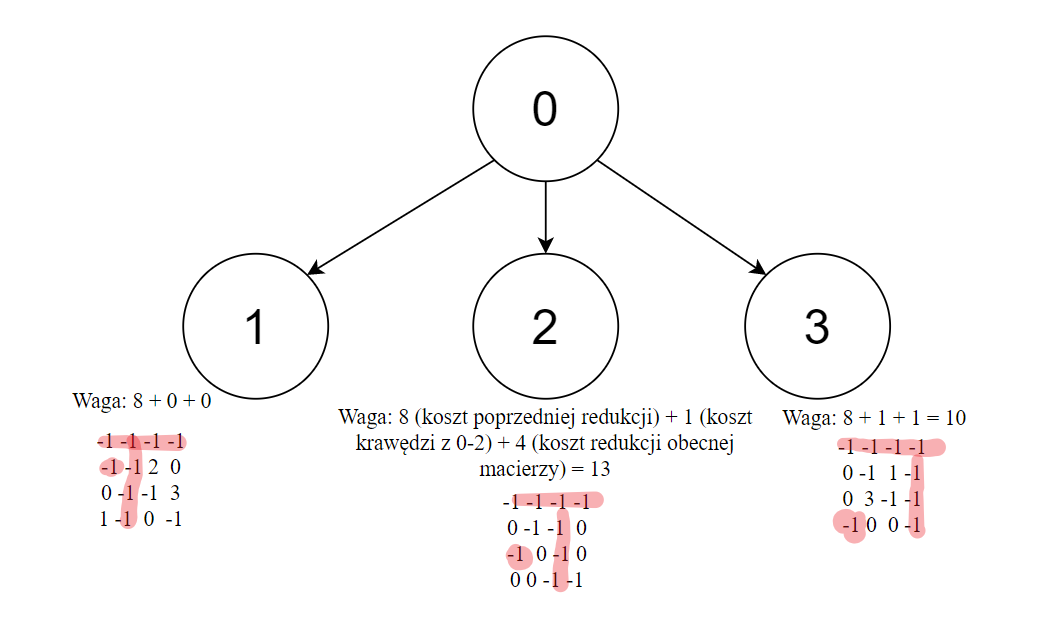
\includegraphics[scale=0.4]{img/graf2.png}
\end{figure}

\newpage
\begin{center}
Rozwijamy macierze dla wierzchołków dostępnych dla ścieżki 0-1:    
\end{center}
\begin{figure}[h]
    \centering
    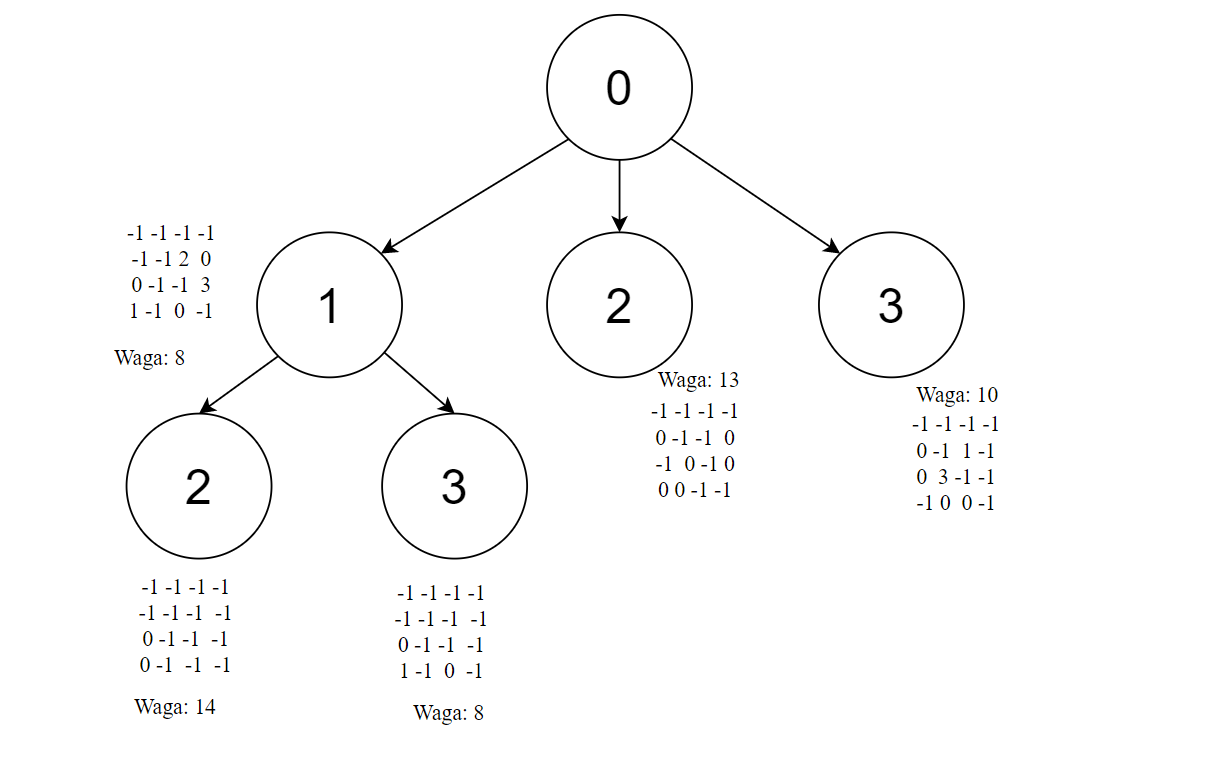
\includegraphics[scale=0.292]{img/graf3.png}
\end{figure}

\begin{center}
    Ponieważ ścieżka 0-1-3 ma długość o jeden mniejszą niż rozmiar macierzy, oraz ma najmniejszą wagę, ostateczną ścieżką będzie 0-1-3-2 (pozostały wierzchołek) - 0(wierzchołek startowy).
\end{center}


\newpage

\section{Pomiary czasu}

\subsection{Sposób pomiaru}
Do pomiarów czasu wykorzystana została klasa Stopwatch z biblioteki $System$. Umożliwia ona dokonania pomiarów z dokładnością do milisekundy.
\subsection{Przebieg}
\begin{enumerate}
    \item Wygeneruj graf (rozmiar podany przez użytkownika).
    \item Wykonaj 50 rozwiązań (bez zapisania wyniku).
    \item Wykonaj 100 rozwiązań zapisując wyniki.
    \item Podaj średnią z zapisanych rozwiązań
\end{enumerate}

W przypadku metody Brute force dla większych macierzy liczba powtórzeń została ograniczona do 10 (bez rozgrzewki).



\section{Wyniki pomiarów}
\subsection{Metoda przeglądu zupełnego}
\subsubsection{Tabela}
\vspace{1cm}
\begin{table}[h]
    \centering
    \begin{tabular}{|c|c|}
    \hline
        rozmiar macierzy & czas [ms] \\ \hline
        8 & 0,2 \\ \hline
        9 & 2,5 \\ \hline
        10 & 28 \\ \hline
        11 & 278 \\ \hline
        12 & 3192,2 \\ \hline
        13 & 38987,4 \\ \hline
        14 & 530580,8 \\ \hline
    \end{tabular}
\end{table}

\subsubsection{Wykres}
\begin{figure}[h]
    \centering
    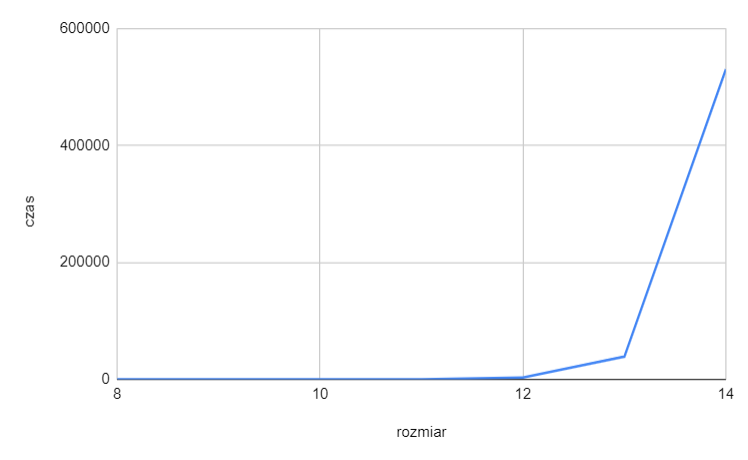
\includegraphics[scale=0.3]{img/wykres1.png}
\end{figure}


\newpage

\subsection{Metoda podziału i ograniczeń}

\subsubsection{Tabela}
\vspace{1cm}
\begin{table}[h]
    \centering
    \begin{tabular}{|c|c|}
    \hline
        rozmiar macierzy & czas [ms]  \\ \hline
        10 & 0,52  \\ \hline
        11 & 0,95  \\ \hline
        12 & 2,28  \\ \hline
        13 & 6,02  \\ \hline
        14 & 17,22  \\ \hline
        15 & 26,27  \\ \hline
        16 & 191,56 \\ \hline
    \end{tabular}
\end{table}

\subsubsection{Wykres}
\begin{figure}[h]
    \centering
    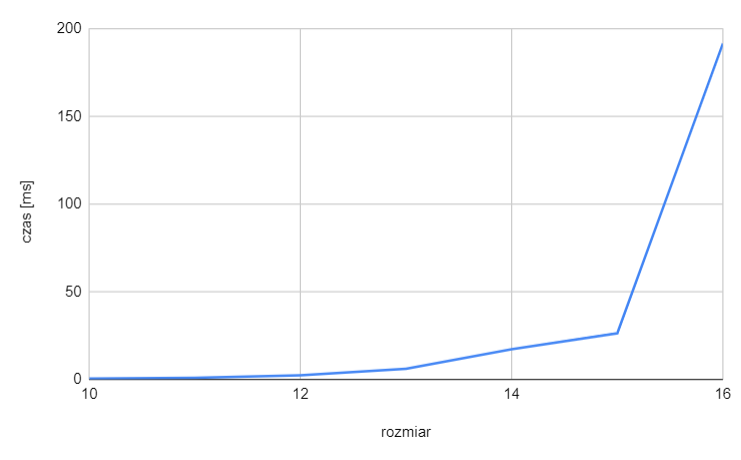
\includegraphics[scale=0.4]{img/wykres2.png}
\end{figure}


\subsection{Porównanie}
\begin{figure}[h]
    \centering
    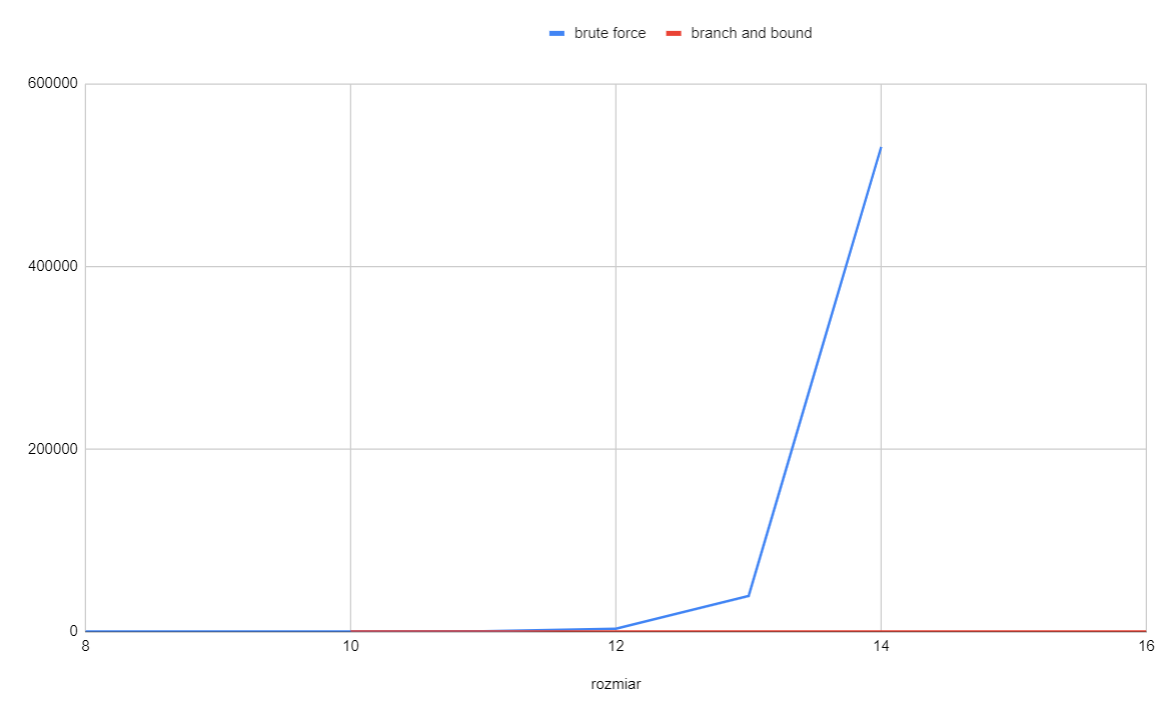
\includegraphics[scale=0.2]{img/wykres3.png}
\end{figure}

\newpage

\section{Wnioski}

Algorytmy zachowywały się zgodnie z oczekiwaniami. Ilość kombinacji do zbadania przez algorytm przeglądu zupełnego bardzo szybko wzrastała, przez co szukanie dla większych rozmiarów problemu stawało się czasochłonne. Niezależnie od instancji problemu, czas obliczeń zawsze był do siebie zbliżony, czego nie można powiedzieć o metodzie podziału i ograniczeń, która w zależnoście od danych początkowych miała bardzo duże wachania w czasie rozwiązania. Ponadto, kiedy daną wejściową był graf nieskierowany, czasy wykonania było często dużo wyższe niż dla grafów skierowanych.


\section{Literatura}

\begin{enumerate}
    \item \url{https://www.interviewbit.com/blog/next-permutation-problem/}
    \item \url{https://www.youtube.com/watch?v=1FEP_sNb62k}
        \item \url{https://iq.opengenus.org/travelling-salesman-branch-bound}
\end{enumerate}

\end{document}
